\documentclass[12pt,twoside]{article}
\usepackage{light}
\usepackage{subfigure}
\usepackage{enumitem}
\usepackage{graphicx}
\hidesolutions
%\showsolutions

%Solutions are currently incorrect
\begin{document}

\begin{problem}{10}
\bparts
\ppart{2} Does the above graph have a Hamiltonian path?

\ppart{2} Does the above graph have a Eulerian path?

\ppart{6} Consider the complete graph on $n$ vertices $K_n$ for odd $n \geq 3$.  Prove that we cannot find a series of Hamiltonian paths in $K_n$ that together cover all the edges of $K_n$.  

\eparts
\end{problem}

%%%%%%%%%%%%%%%%%%%%%%%%%%%%%%%%%%%%%%%%%%%%%%%%%%%%%

%\newpage

%%%%%%%%%%%%%%%%%%%%%%%%%%%%%%%%%%%%%%%%%%%%%%%%%%%%%


\begin{problem}{10}
\bparts
\ppart{3}  Find $7^{100}$ mod $13$.

\ppart{3} Find the inverse of $33$ mod $121$ or prove that no such inverse exists.

\ppart{4} Prove that for any non-zero integers $a, b, c, d$, if $a - c \mid ab + cd$, then $a - c \mid ad + bc$.

\eparts
\end{problem}

%%%%%%%%%%%%%%%%%%%%%%%%%%%%%%%%%%%%%%%%%%%%%%%%%%%%%

%\newpage

%%%%%%%%%%%%%%%%%%%%%%%%%%%%%%%%%%%%%%%%%%%%%%%%%%%%%


\begin{problem}{10}
Suppose we are planning a trip to California for Thanksgiving.  Unfortunately, we are booking our tickets late and so the prices are all really high. Suppose we are given the following list of ticket prices and travel times:

\begin{enumerate}[label=\Alph*]
\item 600 dollars, 9 hours 20 minutes
\item 650 dollars, 8 hours 40 minutes
\item 550 dollars, 9 hours 10 minutes
\item 575 dollars, 8 hours 20 minutes
\item 660 dollars, 9 hours 5 minutes
\end{enumerate}

Our goal is to find the tickets that are the cheapest while minimizing travel time.

\bparts
\ppart{4} Show that the relation of being more expensive and having more travel time creates a partial order for tickets.
\ppart{3} Draw the Hasse diagram for the above tickets with the ticket $i$ is $<$ ticket $j$ if ticket $i$ is both more expensive and has more travel time than ticket $j$.
\ppart{3} Find the maximal elements of the poset.  Is there a maximum element? 
\eparts
\end{problem}

%%%%%%%%%%%%%%%%%%%%%%%%%%%%%%%%%%%%%%%%%%%%%%%%%%%%%

%\newpage

%%%%%%%%%%%%%%%%%%%%%%%%%%%%%%%%%%%%%%%%%%%%%%%%%%%%%


\begin{problem}{10} 
A portion of a computer program consists of a sequence of calculations
where the results are stored in variables, like this:
\[
\begin{array}{rrrcl}
&& \text{Inputs:} &  & x, y \\
\text{Step } 1. & \hspace{0.5in} & a & = & x - 24 \\
2. && b & = & x * a \\
3. && c & = & 3 \\
4. && d & = & y - c \\
5. && e & = & y ** c \\
6. && f & = & e + 1  \\
&& \text{Outputs:} & & b, d, e
\end{array}
\]
A computer can perform such calculations most quickly if the value of
each variable is stored in a \emph{register}, a chunk of very fast
memory inside the microprocessor.  Programming language compilers face
the problem of assigning each variable in a program to a register.
Computers usually have few registers, however, so they must be used
wisely and reused often.  This is called the \emph{register
  allocation} problem.

In the example above, variables $x$ and $y$ must be assigned different
registers, because they hold distinct input values.  Furthermore, $c$
and $d$ must be assigned different registers; if they used the same
one, then the value of $c$ would be overwritten in the fourth step and
we'd get the wrong answer in the fifth step.  On the other hand,
variables $b$ and $d$ may use the same register; we no longer need $b$ and can overwrite the register that holds its
value.  Assume that the computer carries out each step in the order
listed and that each step is completed before the next is begun.

\bparts

\ppart{7} Recast the register allocation problem as a question
about graph coloring.  What do the vertices correspond to?  Construct
the graph corresponding to the example above.

\solution{
There is one vertex for each variable.  An edge between two vertices
indicates that the values of the variables must be stored in different
registers.  We can tell when two variables must be stored in different
registers as follows: classify each appearance of a variable in the
program as either an \emph{assignment} or a \emph{use}.  An appearance
is an \emph{assignment} when the variable is on the left side of an
equation or on the ``Inputs'' line.  An appearance of a variable is a
\emph{use} if the variable is on the right side of
an equation or on the ``Outputs'' line.  The \emph{lifetime} of a variable is the segment of code
extending from the initial assignment of the variable until the last
use.  There is an edge between two variables iff their lifetimes
overlap.

  We are also assuming that all variables are relevant to the Outputs,
  where a variable is \emph{relevant} iff it
  is an Output or is used in an assignment to a relevant variable.
  This is a recursive---not a circular---definition of relevant
  variable!

  Likewise, we assume that all variables are \emph{dependent} on the Inputs, where a variable is
  dependent on the Inputs iff it is an Input or appears in the left
  hand side of an assignment whose right hand side contains a
  dependent variable.
}

\ppart{3} How many registers
do you need?

\solution{
Four registers are needed.

One possible assignment of variables to registers is indicated in the
figure above.  In general, coloring a graph using the minimum number
of colors is quite difficult; no efficient procedure is known.
However, the register allocation problem always leads to an
\term{interval graph}, and optimal colorings for interval graphs are
always easy to find.  This makes it easy for compilers to allocate a
minimum number of registers.
}


%%%%%%%%%%%%%%%%%%%%%%%%%%%%%%%%%%%%%%%%%%%%%%%%%%%%%

\newpage

%%%%%%%%%%%%%%%%%%%%%%%%%%%%%%%%%%%%%%%%%%%%%%%%%%%%%


\begin{problem}{10} 
Use the web graph below to answer parts (a), (b), and (c) of this question. The pagerank of vertex $i$ can be written as $p_i$. 

\begin{figure}[!ht]
\begin{center}
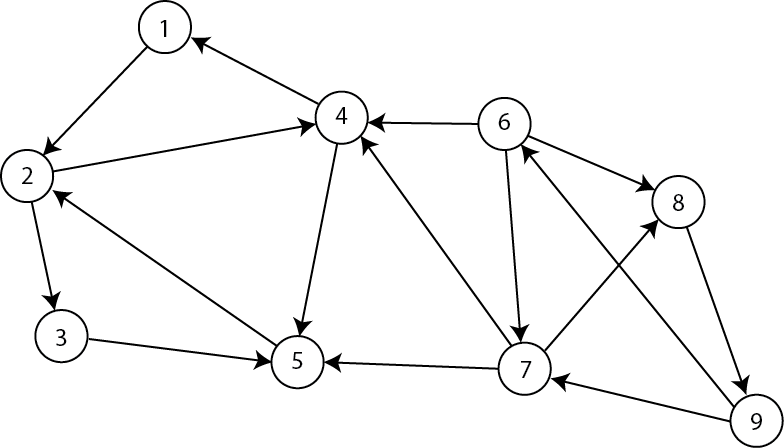
\includegraphics[width=12cm]{pagerank.png}\end{center}
\caption{Web Graph}
\end{figure}


\bparts

\ppart{2} For $\vec{p}~'$ in terms of $\vec{p}$ can be written as a matrix product: $\vec{p}' = W\vec{p}$, for some matrix $W$, which is the \emph{update matrix}. Find the update matrix.

\ppart{2} Which (if any) of the vertices of the web graph above will have PageRank value tending to zero if we run the PageRunk algorithm for many (let's say 200,000) iterations?

\ppart{6} Suppose we remove all the vertices that you found in part b from our Web Graph along with all corresponding edges from those vertices and consider the remaining graph $G$.  Find the stationary distribution across the nodes assuming that each node in $G$ starts with a value of $\frac{1}{5}$.  

\textbf{Note}: If you are not confident about your answer in part b, feel free to instead find the stationary distribution for the directed triangle formed by vertices 1, 2, 4 of the Web Graph.  Again assume each of the nodes 1, 2, 4 starts with inital PageRank value $\frac{1}{3}$.  

\eparts
\end{problem}

\eparts
\end{problem}
\end{document}
